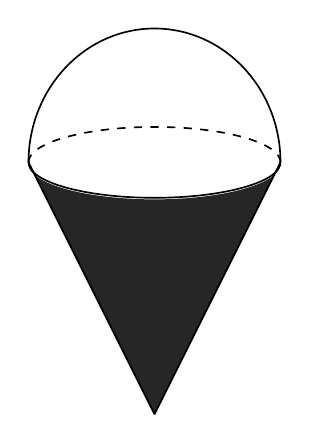
\begin{tikzpicture}[line width=.6pt]
% ice-cream cone: black cone below, hemisphere above, shared rim ellipse
\coordinate (apex) at (0,-3.2);
\coordinate (rimL) at (-1.6,0);
\coordinate (rimR) at (1.6,0);
\def\rimy{0.45}
% cone body (gray block per spec, original solid black)
\fill[black!85] (apex) -- (rimL) -- (rimL) ++(0,-0.02) arc[x radius=1.6, y radius=\rimy, start angle=180, end angle=360] -- (apex) -- cycle;
\draw (apex) -- (rimL);
\draw (apex) -- (rimR);
% rim: front solid (cone top edge), back dashed (hemisphere interior)
\draw (rimL) arc[x radius=1.6, y radius=\rimy, start angle=180, end angle=360];
\draw[dashed] (rimL) arc[x radius=1.6, y radius=\rimy, start angle=180, end angle=0];
% hemisphere dome solid
\draw (rimL) arc[x radius=1.6, y radius=1.7, start angle=180, end angle=0];
\end{tikzpicture}
